%
% Autor: Bartłomiej Kurosz
% bartek.kurosz@gmail.com
%-------------------------------------
% Definicja klasy dokumentu
\documentclass[12pt,a4paper]{article}

%------------------------------------
% 			Pakiety
\usepackage[utf8x]{inputenc}
\usepackage{ucs}
\usepackage[MeX]{polski}
\usepackage{fancyhdr}
\usepackage{amsfonts}
\usepackage{amssymb}
\usepackage{subfig}
\usepackage{supertabular}
\usepackage{array}
\usepackage{tabularx}
\usepackage{hhline}
\usepackage{tabulary}
\pagestyle{fancy}

%---------------------------------------
% 		Dodanie strony tytulowej do dokumentu
\usepackage{graphicx}
\usepackage[hidelinks]{hyperref}

\renewcommand{\maketitle}{\begin{titlepage}

\begin{center}

\includegraphics[scale=1]{title/logo.png}
\vspace*{1cm}
\noindent \rule{\linewidth}{0.4mm}
\LARGE \textsc{Praktyczne wprowadzenie do systemu składu tekstu \LaTeX} % Tutaj należy umieścić tytuł projektu 
\vspace*{0.5cm}
\rule{\linewidth}{0.4mm}
\vspace*{2cm}

\large
\textsc{Bartłomiej Kurosz} \\ % W tym miejscu należy zamieścić 


\vspace*{3cm}
\textsc{Koło Naukowe Robotyków KoNaR }\\
\textsc{\url{www.konar.pwr.edu.pl}}\\
\textsc{\today}\\
\end{center}
\end{titlepage}
\newpage
} % W tym pliku należy w odpowiednim miejscu wpisać członków zespołu, tytul itp.

%-----------------------------------------
% 		Poczatek dokumentu
\begin{document}
\maketitle % dodanie strony tytulowej na poczatku
\tableofcontents % dodanie spisu tresci
\newpage % przejscie do nowej strony

%------------------------------------------
%				Dokument wlasciwy
\section{Wstęp}

Niniejszy dokument powstał na potrzeby Warsztatów Robotycznych organizowanych w ramach rekrutacji do \emph{Koła Naukowego Robotyków KoNaR}. Dokument zawiera informacje dotyczące praktycznego wykorzystania elementów systemu składu tekstu \LaTeX. Przedstawiono tu zbiór przykładów, 

W razie problemów czy niejasności proszę kontaktować się z autorem pod adresem \emph{bartek.kurosz@gmail.com}.


\section{Instalacja środowiska}
W tej sekcji przedstawiono przykładowy sposób instalacji dystrybucji systemu \LaTeX oraz programu TexMaker, będącego zintegrowanym środowiskiem programistycznym do tworzenia dokumentów.
\subsection{Instalacja w systemie Linux}
Instalacja dystrybucji \LaTeX\\
\texttt{sudo apt-get install texlive-full} \\\\
%
Instalacja środowiska TexMaker\\
\texttt{sudo apt-get install texmaker}\\\\
%
Instalacja języka polskiego w systemie \LaTeX\\
\texttt{sudo apt-get install texlive-lang-polish}

\subsection{Instalacja w systemie Windows}
Instalacja dystrybucji \LaTeX --- MikTex --- do pobrania np. pod poniższym adresem\\
\href{http://miktex.org/download}{\texttt{http://miktex.org/download}}\\\\
%
Instalacja środowiska TexMaker --- 
do pobrania np. pod poniższym adresem\\
\href{http://www.xm1math.net/texmaker/download.html}{\texttt{http://www.xm1math.net/texmaker/download.html}}




\section{How To \LaTeX}

\subsection{Podstawy}

Pisząc zwykły tekst można sobie pozwolić na dowolną       ilość     spacji 
pomiędzy         słowami.          \LaTeX~                wszystko           sformatuje 
                                        tak,                     żeby było poprawnie.
Można również używać jednokrotnego znaku enter, aby przedzielić tekst
kiedy
uznamy 
to
za
wygodne
dla
przejrzystości
tekstu.

Pozostawienie jednej pustej linii w kodzie źródłowym, oznacza rozpoczęcie nowego akapitu.

\subsection{Struktura dokumentu}

Mechanizm tworzenia struktury dokumentu jest bardzo prosty i intuicyjny.
W zależności od typu dokumentu, największymi częściami będą sekcje lub rozdziały (section, chapter).
Sekcje można dzielić na podsekcje (subsection),
\subsubsection{Podsekcje}
a podsekcje na podpodsekcje (subsubsection).
W każdej strukturze organizacyjnej można utworzyć kilka bytów niższych w hierarchii, jak poniżej.
\subsubsection{Podział drugi}
\subsubsection{Jeszcze jedna podpodsekcja}

W razie potrzeby, można zejść jeszcze niżej i użyć paragrafów (paragraph)
\paragraph{Paragraf o paragrafie}
Paragrafy po pierwsze nie będą występować w spisie treści (w przeciwieństwie do wszystkich będących wyżej w strukturze dokumentu), a po drugie po nazwie paragrafu nie pojawi się nowa linia.

\paragraph{Jeszcze jeden niepotrzebny paragraf} Tak tylko żeby zilustrować mechanizm.

\subsection{Komendy}
Większość komend specjalnych w systemie \LaTeX~zaczyna się od znaku backslash. Aby uwidocznić pewne cechy tekstu, można stosować komendy takie jak \textbf{bold} czy \textit{italic}.
(TexMaker zawiera wiele skrótów klawiszowych, i tak powyższe komendy w kodzie źródłowym można dodać za
pomocą klawiszy Ctrl+B oraz Ctrl+I.

\subsection{Dodawanie obrazków}

\LaTeX~ ułatwia proces wstawiania obrazków, automatycznie realizując odpowiednie pozycjonowanie. Na rysunku \ref{fig:flash} przedstawiono robota Flash, który powstał na Wydziale Elektroniki.
%
\begin{figure}[tp]
\centering
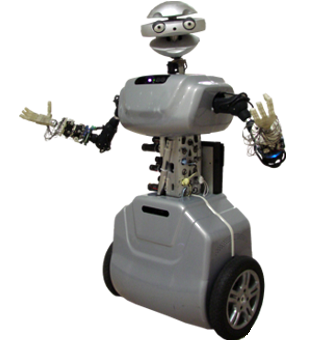
\includegraphics[width=0.8\textwidth]{figures/Flash.png}
\caption{Robot Flash \label{fig:flash}}
\end{figure}


\subsection{Dodawanie zestawień obrazków}
Istnieje również łatwy sposób tworzenia zestawień rysunków, bez konieczności skalowania każdego obrazka ręcznie. Przykład pokazano na rysunku \ref{fig:roboty}.
%
\begin{figure}[tp]
\centering

    \subfloat[Asimo\label{subfig:Asimo}]{%
      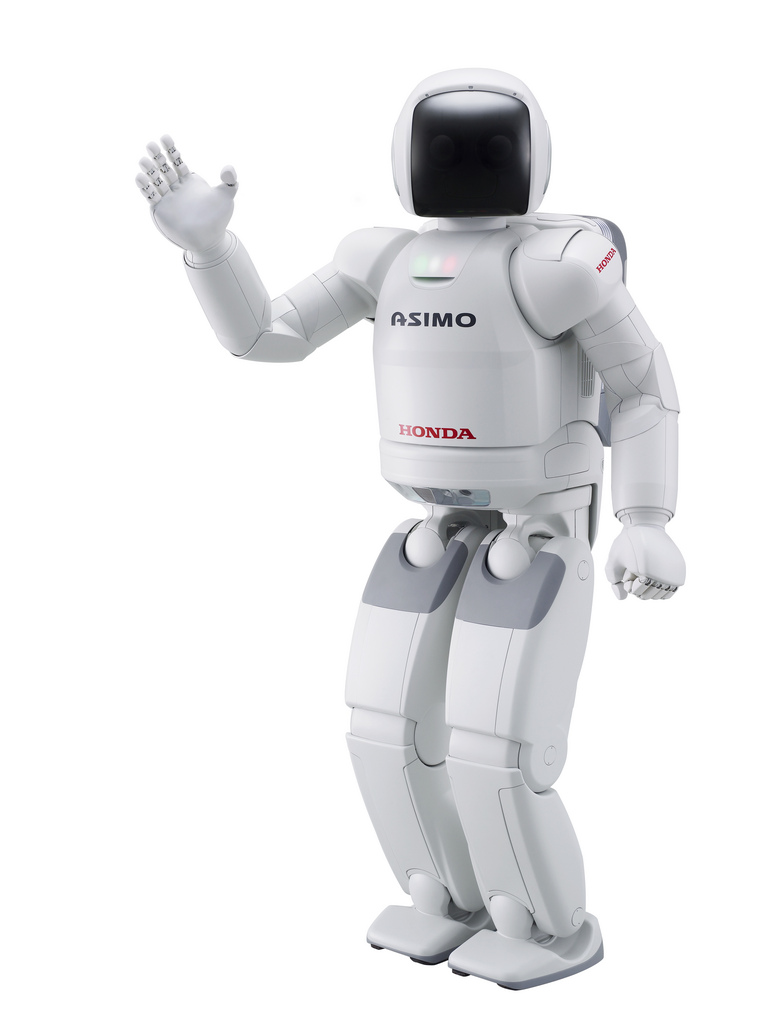
\includegraphics[width=0.3\textwidth]{figures/Asimo.jpg}
    } %Miedzy tymi obrazkami nie ma przerwy, wiec beda zestawione poziomo
    \hspace{0.4cm}
    \subfloat[Atlas\label{subfig:Atlas}]{%
      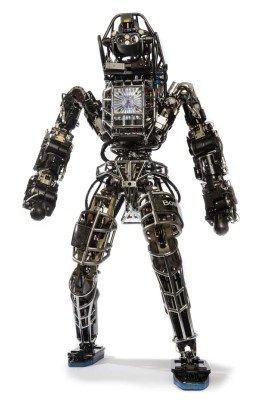
\includegraphics[width=0.3\textwidth]{figures/Atlas.jpg}
    }%Ponizej jest przerwa, wiec nastapi przejscie do nowej linii


    \subfloat[Curiosity\label{subfig:curiosity}]{%
      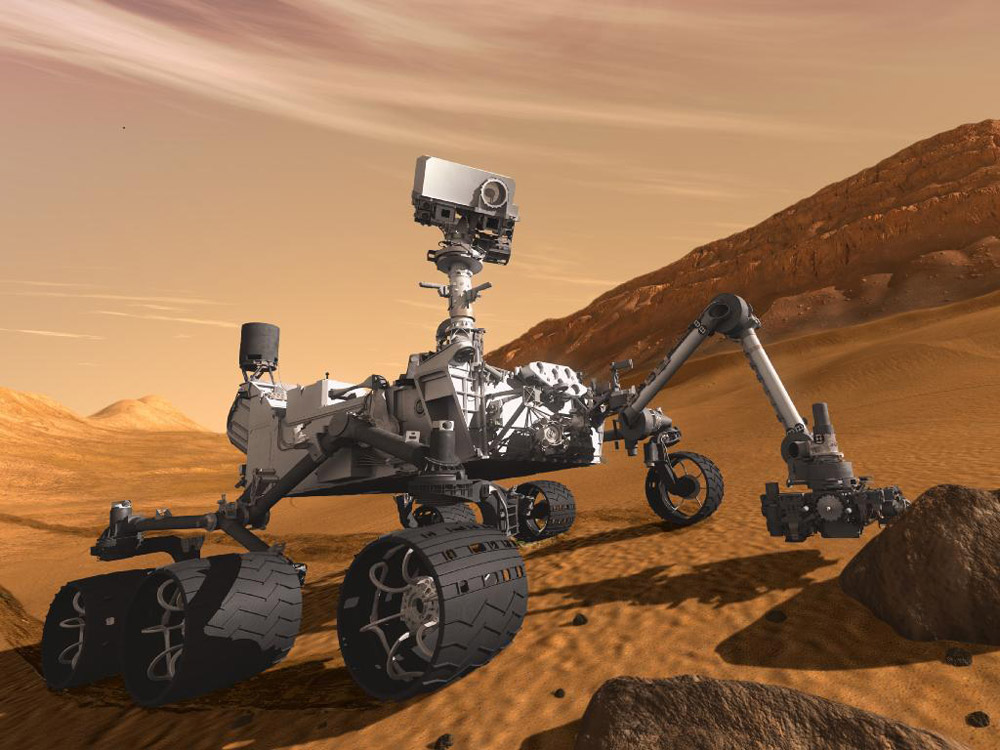
\includegraphics[width=0.3\textwidth]{figures/Curiosity.jpg}
    }
    \hspace{0.4cm}
    \subfloat[Nao\label{subfig:nao}]{%
      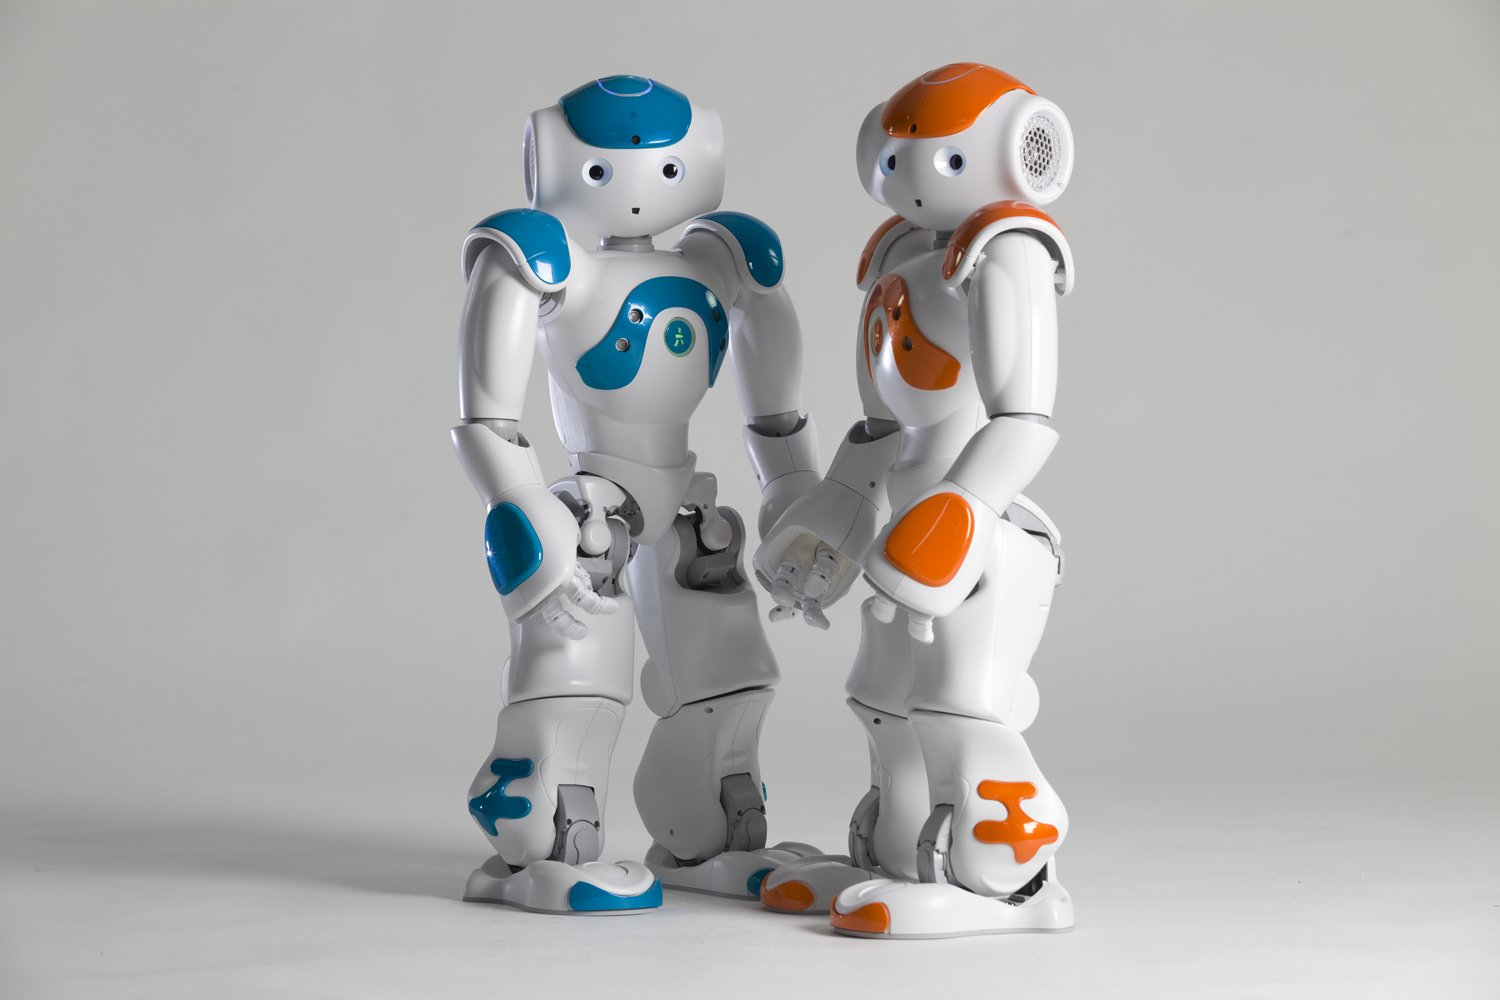
\includegraphics[width=0.3\textwidth]{figures/NAO.jpg}
    }

    \subfloat[Wildcat\label{subfig:wildcat}]{%
      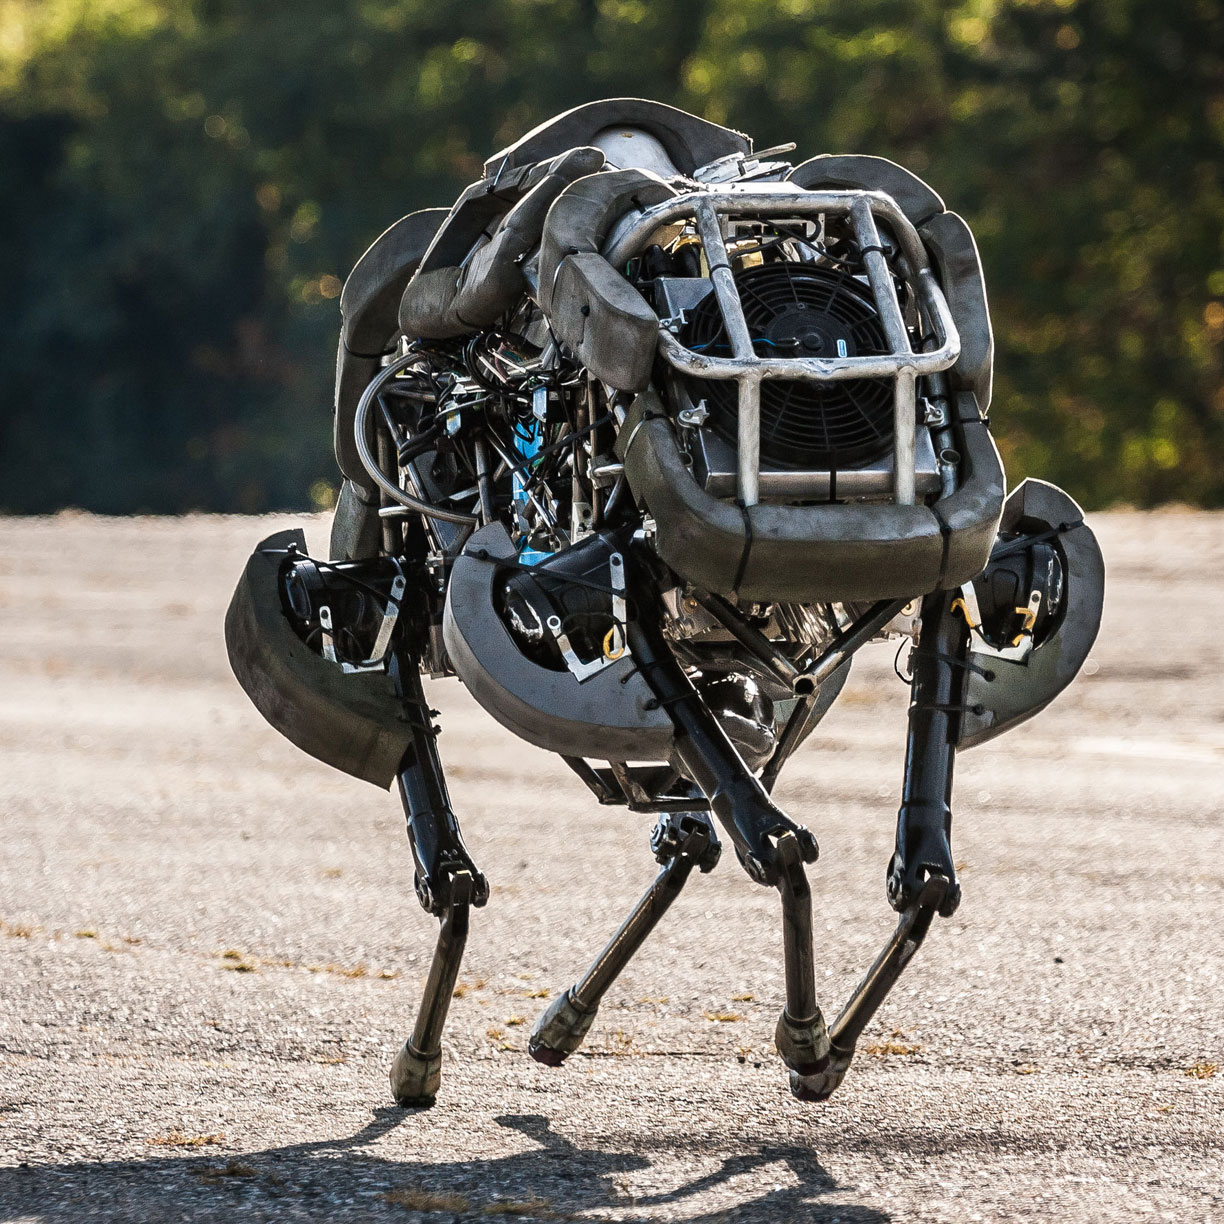
\includegraphics[width=0.3\textwidth]{figures/Wildcat.jpg}
    }
    \hspace{0.4cm}
    \subfloat[Baxter\label{subfig:baxter}]{%
      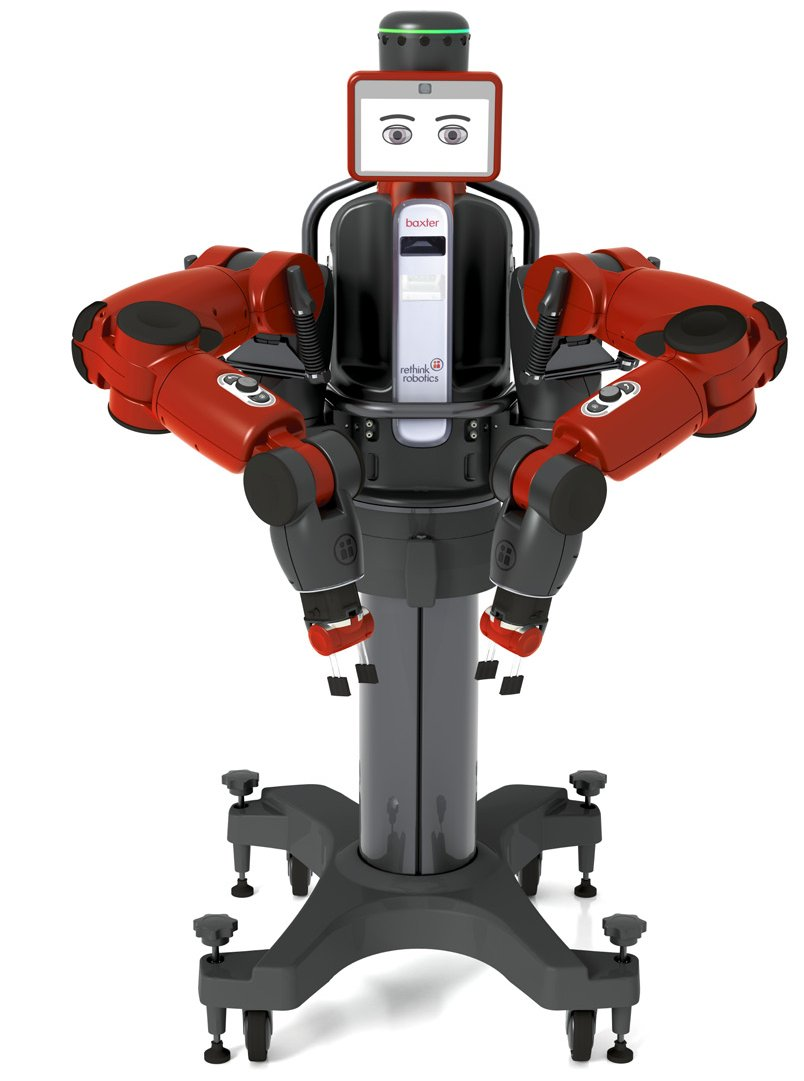
\includegraphics[width=0.3\textwidth]{figures/Baxter.jpg}
    }
    
    \caption{Zestawienie wybranych najważniejszych robotów ostatnich kilku lat}
    \label{fig:roboty}
  \end{figure}%




\section{Tabele}
Tabele można tworzyć na wiele różnych sposobów. W tabeli \ref{zestawienie} zaprezentowano jeden z nich.
%
\begin{table}[tp]
\centering
\caption{Zestawienie wyników pięciu najszybszych robotów klasy LineFollower na zawodach Robotic Arena 2016 \label{zestawienie}}
\begin{tabulary}{\textwidth}
{|p{0.3\textwidth}|p{0.2\textwidth}|p{0.3\textwidth}|}
\hline
\textbf{Nazwa robota} & \textbf{Pozycja} & \textbf{Czas przejazdu [s]} \\
\hline
Pika & 1 & 31.609\\
\hline
SkyLake & 2 & 34.374\\
\hline
Bullet & 3 & 34.672\\
\hline
Camel & 4 & 51.525\\
\hline
\end{tabulary}
\end{table}%
%
Składnia tabeli jest mało wygodna w użyciu, szczególnie dla większych zestawów danych. Aby ułatwić proces tworzenia tabel, można posłużyć się generatorami tabel do systemu \LaTeX~ dostępnymi w sieci.
%

\section{Listy}
%
Prostym i skutecznym sposobem na przedstawienie informacji jest wypunktowanie bądź numeracja.
%
\begin{itemize}
%
\item Tak wygląda środowisko \emph{itemize}.
%
\item Przy każdym elemencie dodawana jest kropka.
%
\item To już ostatnia w tym przykładzie.
%
\end{itemize}
%
Chcąc zaznaczyć fakt, że kolejność jest istotna, można posłużyć się środowiskiem \emph{enumerate}.
%
\begin{enumerate}
%
\item Tak właśnie prezentuje się środowisko \emph{enumerate},
%
\item numerując po kolei każdy z elementów,
%
\item dodany do listowania.
%
\end{enumerate}
%
\section{Wzory matematyczne}
Wszystkie wyrażenia matematyczne powinny być zapisywane w trybie matematycznym.
Najprostszym jest tryb wierszowy, przydatny kiedy chcemy po prostu przypomnieć w tekście, że $E=mc^2$. \LaTeX~ dostarcza tekstowy mechanizm tworzenia wyrażeń matematycznych, pozwalający w prosty sposób tworzyć rzeczy takie jak indeksy dolne $a_1$, górne $x^2$, ułamki $\frac{1}{2}$ oraz wiele innych funkcji. 

Chcąc wyodrębnić wzór, należy użyć środowiska equation.

\begin{equation}
\label{eq:calka}
s  = \int_{a}^{b} x^2 dx
\end{equation}

Co więcej, do równań można się odnosić tak samo jak do obrazków czy tabel, tak jak w przypadku równania \ref{eq:calka}.

\section{Cytowania}
Warto także wskazać na czym oparło się swoją pracę,bądź gdzie można znaleźć jakieś wartościowe informacje. Na przykład:
podczas tworzenia robota wiele informacji znaleziono na portalu Forbot \cite{forbot}.

Istnieje rzetelny i godny polecenia portal internetowy \cite{ieee}, na którym co tydzień w piątek prezentowane jest zestawienie ciekawych filmów robotycznych z minionego tygodnia.

\section{Gdzie szukać informacji?}
Wartym uwagi dokumentem jest \quotedblbase Nie za krótkie wprowadzenie do systemu \LaTeX\textquotedblright 

Nieco bardziej skondensowanym i przystępnym źródłem wiedzy jest strona ShareLatex ---
\href{https://www.sharelatex.com/learn/}{https://www.sharelatex.com/learn/}


\end{document}